\documentclass[12pt, titlepage]{article}

\usepackage{fullpage}
\usepackage[round]{natbib}
\usepackage{multirow}
\usepackage{booktabs}
\usepackage{tabularx}
\usepackage{longtable}
\usepackage{graphicx}
\usepackage{tikz}
\usetikzlibrary{arrows.meta,positioning}
\usepackage{float}
\usepackage{hyperref}
\hypersetup{
    colorlinks,
    citecolor=blue,
    filecolor=black,
    linkcolor=red,
    urlcolor=blue
}

\input{../../Comments.text}
\input{../../Common.text}

\newcounter{acnum}
\newcommand{\actheacnum}{AC\theacnum}
\newcommand{\acref}[1]{AC\ref{#1}}

\newcounter{ucnum}
\newcommand{\uctheucnum}{UC\theucnum}
\newcommand{\uref}[1]{UC\ref{#1}}

\newcounter{mnum}
\newcommand{\mthemnum}{M\themnum}
\newcommand{\mref}[1]{M\ref{#1}}

\begin{document}

\title{Module Guide for \progname{}} 
\author{\authname}
\date{\today}

\maketitle

\pagenumbering{roman}

\section{Revision History}

\begin{tabularx}{\textwidth}{p{3cm}p{2cm}X}
\toprule {\bf Date} & {\bf Version} & {\bf Notes}\\
\midrule
November 13, 2026 & -1 & Initial module decomposition and anticipated changes.\\
November 13, 2026 & -1 & Requirements traceability, interfaces, and supporting design sections.\\
\bottomrule
\end{tabularx}

\newpage

\section{Reference Material}

This section defines terminology used throughout the module decomposition.

\subsection{Abbreviations and Acronyms}
\renewcommand{\arraystretch}{1.2}
\begin{tabularx}{\textwidth}{@{}lX@{}}
\toprule
\textbf{Symbol} & \textbf{Description}\\
\midrule
AC & Anticipated change\\
API & Application programming interface\\
CI & Continuous integration\\
DAG & Directed acyclic graph\\
M & Module\\
MG & Module Guide\\
MIS & Module Interface Specification\\
OS & Operating system\\
PoC & Proof of concept\\
SRS & Software Requirements Specification\\
UC & Unlikely change\\
UI & User interface\\
\bottomrule
\end{tabular}

\newpage

\tableofcontents

\listoftables

\listoffigures

\newpage

\pagenumbering{arabic}

\section{Introduction}

Decomposing a system into modules is a commonly accepted approach to developing
software.  A module is a work assignment for a programmer or programming
team~\citep{ParnasEtAl1984}.  We advocate a decomposition
based on the principle of information hiding~\citep{Parnas1972a}.  This
principle supports design for change, because the ``secrets'' that each module
hides represent likely future changes.  For LingoLyrics, design for change separates decisions that may evolve
independently: platform integration, song-map representation, lyric
synchronization, lesson authoring, language processing, and vocabulary
transfer. The system comprises an iOS/Android learner application and a
browser-based song-map editor. Both depend on one versioned lesson format
and common validation rules. Modules hide these decisions so that changing a
language-processing library or Anki transfer method does not require
rewriting unrelated user workflows.  

Our design follows the rules layed out by \citet{ParnasEtAl1984}, as follows:
\begin{itemize}
\item System details that are likely to change independently should be the
  secrets of separate modules.
\item Each data structure is implemented in only one module.
\item Any other program that requires information stored in a module's data
  structures must obtain it by calling access programs belonging to that module.
\end{itemize}

After completing the first stage of the design, the Software Requirements
Specification (SRS), the Module Guide (MG) is developed~\citep{ParnasEtAl1984}. The MG
specifies the modular structure of the system and is intended to allow both
designers and maintainers to easily identify the parts of the software.  The
potential readers of this document are as follows:

\begin{itemize}
\item New project members: This document can be a guide for a new project member
  to easily understand the overall structure and quickly find the
  relevant modules they are searching for.
\item Maintainers: The hierarchical structure of the module guide improves the
  maintainers' understanding when they need to make changes to the system. It is
  important for a maintainer to update the relevant sections of the document
  after changes have been made.
\item Designers: Once the module guide has been written, it can be used to
  check for consistency, feasibility, and flexibility. Designers can verify the
  system in various ways, such as consistency among modules, feasibility of the
  decomposition, and flexibility of the design.
\end{itemize}

The authoritative requirements are in the
\href{https://github.com/rhea333/LingoLyrics/blob/main/docs/SRS-Volere/SRS.tex}
{Volere SRS}. The
\href{https://github.com/rhea333/LingoLyrics/blob/main/docs/DevelopmentPlan/DevelopmentPlan.tex}
{Development Plan} gives milestones and initial component owners. The
accompanying Module Interface Specification (MIS) defines each module's
public contract.

Section~\ref{SecChange} identifies design changes; Section~\ref{SecMH}
names the modules; Section~\ref{SecConnection} explains architectural
decisions; Section~\ref{SecMD} documents module secrets and services;
Section~\ref{SecTM} traces requirements and changes; and
Section~\ref{SecUse} documents dependencies. The remaining sections cover
user interfaces, communication, persistence, implementation planning, and
generative AI use.

\section{Anticipated and Unlikely Changes} \label{SecChange}

This section lists possible changes to the system. According to the likeliness
of the change, the possible changes are classified into two
categories. Anticipated changes are listed in Section \ref{SecAchange}, and
unlikely changes are listed in Section \ref{SecUchange}.

\subsection{Anticipated Changes} \label{SecAchange}

Anticipated changes are the source of the information that is to be hidden
inside the modules. Ideally, changing one of the anticipated changes will only
require changing the one module that hides the associated decision. The approach
adapted here is called design for
change.

\begin{description}
\item[\refstepcounter{acnum} \actheacnum \label{acPlatforms}:] The mobile and
  desktop operating systems and platform APIs supported by the learner
  application and creator editor.
\item[\refstepcounter{acnum} \actheacnum \label{acSongMap}:] The structure,
  fields, and versioning rules of the shared song-map format.
\item[\refstepcounter{acnum} \actheacnum \label{acAudio}:] The audio playback
  technology and the method used to obtain playback position for lyric
  synchronization.
\item[\refstepcounter{acnum} \actheacnum \label{acAuthoring}:] The creator
  workflow and the controls used to enter and edit lyric timing, translations,
  transliterations, and annotations.
\item[\refstepcounter{acnum} \actheacnum \label{acLanguage}:] The supported
  languages and the language-specific text processing needed to present them.
\item[\refstepcounter{acnum} \actheacnum \label{acAnki}:] The supported method
  for transferring selected vocabulary, including the mapping to Anki note
  fields.
\end{description}

\subsection{Unlikely Changes} \label{SecUchange}

The module design should be as general as possible. However, a general system is
more complex. Sometimes this complexity is not necessary. Fixing some design
decisions at the system architecture stage can simplify the software design. If
these decision should later need to be changed, then many parts of the design
will potentially need to be modified. Hence, it is not intended that these
decisions will be changed.

\begin{description}
\item[\refstepcounter{ucnum} \uctheucnum \label{ucProduct}:] The product will
  continue to provide a mobile learner experience and a companion web-based
  authoring workflow, rather than combining both workflows into a single
  platform.
\item[\refstepcounter{ucnum} \uctheucnum \label{ucStreaming}:] The initial
  product will not integrate with streaming services or provide a production
  music catalogue; lessons use audio and song-map content supplied by creators.
\item[\refstepcounter{ucnum} \uctheucnum \label{ucContentRights}:] The product
  will not acquire or distribute copyrighted recordings or lyrics without
  authorization. Initial lesson content will be team-created, public-domain, or
  appropriately licensed.
\end{description}

\section{Module Hierarchy} \label{SecMH}

This section provides an overview of the module design. Modules are summarized
in a hierarchy decomposed by secrets in Table \ref{TblMH}. The modules listed
below, which are leaves in the hierarchy tree, are the modules that will
actually be implemented.

\begin{description}
\item [\refstepcounter{mnum} \mthemnum \label{mHH}:] Platform and Media Adapter
\item [\refstepcounter{mnum} \mthemnum \label{mLearner}:] Learner Lesson Interface
\item [\refstepcounter{mnum} \mthemnum \label{mEditor}:] Song Map Authoring Interface
\item [\refstepcounter{mnum} \mthemnum \label{mValidate}:] Song Map Validation Module
\item [\refstepcounter{mnum} \mthemnum \label{mAnki}:] Vocabulary Handoff Module
\item [\refstepcounter{mnum} \mthemnum \label{mMap}:] Shared Song Map Format Module
\item [\refstepcounter{mnum} \mthemnum \label{mSync}:] Playback Synchronization Module
\item [\refstepcounter{mnum} \mthemnum \label{mLanguage}:] Language Text Processing Module
\end{description}


\begin{table}[h!]
\centering
\begin{tabular}{p{0.3\textwidth} p{0.6\textwidth}}
\toprule
\textbf{Level 1} & \textbf{Level 2}\\
\midrule

\multirow{1}{0.3\textwidth}{Hardware-Hiding Module} & Platform and Media Adapter\\
\midrule

\multirow{4}{0.3\textwidth}{Behaviour-Hiding Module} & Learner Lesson Interface\\
& Song Map Authoring Interface\\
& Song Map Validation Module\\
& Vocabulary Handoff Module\\
\midrule

\multirow{3}{0.3\textwidth}{Software Decision Module} & Shared Song Map Format Module\\
& Playback Synchronization Module\\
& Language Text Processing Module\\
\bottomrule

\end{tabular}
\caption{Module Hierarchy}
\label{TblMH}
\end{table}

\section{Connection Between Requirements and Design} \label{SecConnection}

The design of the system is intended to satisfy the requirements developed in
the SRS. In this stage, the system is decomposed into modules. The connection
between requirements and modules is listed in Table~\ref{TblRT}.

The learner and editor share the same song-map representation
(\mref{mMap}) and validation service (\mref{mValidate}) to satisfy
FR16 and IN2: import and export must agree on validity. The editor
owns segmentation suggestions and creator verification, while the
learner displays the stored results without running a tokenizer (IN4).
Synchronization is calculated from reported audio position rather than
a parallel timer (IN1). Anki transport and note-field mapping are
isolated in \mref{mAnki}; the learner interface does not depend on a
particular Anki integration method (LC1). These decisions are
reflected in the allocation tables of Section~\ref{SecTM}.

\section{Module Decomposition} \label{SecMD}

Modules are decomposed according to the principle of ``information hiding''
proposed by \citet{ParnasEtAl1984}. The \emph{Secrets} field in a module
decomposition is a brief statement of the design decision hidden by the
module. The \emph{Services} field specifies \emph{what} the module will do
without documenting \emph{how} to do it. For each module, a suggestion for the
implementing software is given under the \emph{Implemented By} title. If the
entry is \emph{OS}, this means that the module is provided by the operating
system or by standard programming language libraries.  \emph{\progname{}} means the
module will be implemented by the \progname{} software.

Only the leaf modules in the hierarchy have to be implemented. If a dash
(\emph{--}) is shown, this means that the module is not a leaf and will not have
to be implemented.

\subsection{Hardware Hiding Modules (\mref{mHH})}

\begin{description}
\item[Secrets:] The platform-specific interfaces for audio playback, playback
  position, and access to lesson files.
\item[Services:] Provides the learner and editor applications with audio
  playback, playback position, and platform file access without exposing
  platform-specific APIs to those applications.
\item[Implemented By:] Expo Audio and operating-system APIs in the learner app;
  browser audio and file APIs in the editor.
\item[Type of Module:] Library
\end{description}

\subsection{Behaviour-Hiding Modules}

\begin{description}
\item[Secrets:]The contents of the required behaviours.
\item[Services:]Includes programs that provide externally visible behaviour of
  the system as specified in the software requirements specification (SRS)
  documents. This module serves as a communication layer between the
  hardware-hiding module and the software decision module. The programs in this
  module will need to change if there are changes in the SRS.
\item[Implemented By:] --
\end{description}

\subsubsection{Learner Lesson Interface (\mref{mLearner})}

\begin{description}
\item[Secrets:] The interaction and presentation design for studying a song,
  including synchronized lyrics and contextual support.
\item[Services:] Presents a lesson, follows the audio with the relevant lyric
  line, and displays translations, transliterations, and annotations when
  learners select lyric content.
\item[Implemented By:] React Native with Expo.
\item[Type of Module:] Abstract Object
\end{description}

\subsubsection{Song Map Authoring Interface (\mref{mEditor})}

\begin{description}
\item[Secrets:] The creator workflow and editor interaction design for preparing
  lesson content.
\item[Services:] Lets creators enter and edit audio references, timed lyrics,
  translations, transliterations, annotations, and language metadata, and
  produces a song map for learner use.
\item[Implemented By:] React web application.
\item[Type of Module:] Abstract Object
\end{description}

\subsubsection{Song Map Validation Module (\mref{mValidate})}

\begin{description}
\item[Secrets:] The validation rules and the way validation failures are
  reported to a creator.
\item[Services:] Determines whether a song map conforms to the shared format
  and reports invalid or missing map data to the editor.
\item[Implemented By:] TypeScript and JSON Schema.
\item[Type of Module:] Library
\end{description}

\subsubsection{Vocabulary Handoff Module (\mref{mAnki})}

\begin{description}
\item[Secrets:] The selected Anki transfer mechanism and the mapping of a
  selected vocabulary item to the destination note fields.
\item[Services:] Transfers a learner-selected term, translation, and context
  to the learner's Anki workflow, or provides an export that can be imported
  into Anki.
\item[Implemented By:] TypeScript; the specific API or export mechanism remains
  a development decision.
\item[Type of Module:] Library
\end{description}


\subsection{Software Decision Module}

\begin{description}
\item[Secrets:] The design decision based on mathematical theorems, physical
  facts, or programming considerations. The secrets of this module are
  \emph{not} described in the SRS.
\item[Services:] Includes data structure and algorithms used in the system that
  do not provide direct interaction with the user. 
  % Changes in these modules are more likely to be motivated by a desire to
  % improve performance than by externally imposed changes.
\item[Implemented By:] --
\end{description}

\subsubsection{Shared Song Map Format Module (\mref{mMap})}

\begin{description}
\item[Secrets:] The song-map data structure, field definitions, and serialized
  representation shared by the learner application and editor.
\item[Services:] Defines the common representation for audio references,
  timed lyrics, translations, transliterations, annotations, and language
  metadata, and makes that representation available to the applications and
  validation module.
\item[Implemented By:] Shared TypeScript types and a versioned JSON Schema.
\item[Type of Module:] Abstract Data Type
\end{description}

\subsubsection{Playback Synchronization Module (\mref{mSync})}

\begin{description}
\item[Secrets:] The decision procedure that associates the current audio
  position with the lyric line or word to present.
\item[Services:] Given playback position and song-map timing data, identifies
  the lyric content that should be active in the lesson view.
\item[Implemented By:] Shared TypeScript logic.
\item[Type of Module:] Library
\end{description}

\subsubsection{Language Text Processing Module (\mref{mLanguage})}

\begin{description}
\item[Secrets:] The language-specific text processing decisions, including
  segmentation and reading generation where required.
\item[Services:] Supplies language-aware text processing needed to present
  supported lyrics and word-level learning content.
\item[Implemented By:] TypeScript language-processing libraries; the initial
  Japanese segmentation candidate is kuromoji.js.
\item[Type of Module:] Library
\end{description}

\section{Traceability Matrix} \label{SecTM}

Table~\ref{TblRT} assigns every numbered requirement in the
\href{https://github.com/rhea333/LingoLyrics/blob/main/docs/SRS-Volere/SRS.tex}
{Volere SRS} to responsible modules. The first, bold module is the
primary owner of the capability; the other modules provide supporting
services. The table covers all numbered functional and nonfunctional
requirements, including the mandated constraints (MC1--MC3).
No module is unassigned, and every SRS requirement has a primary
responsible module. The mapping expresses responsibility, not a promise
that the implementation is already complete.

Some requirements are verified at the project level rather than by
one runtime operation. MC1 and MC2 constrain technology choices;
MS1, MS2, and IM3 require CI checks; OE5 concerns release tags.
These are allocated to the affected modules in Table~\ref{TblRT},
but the build/release workflow must enforce them. They are not
interpreted as additional public methods of those modules.

\small
\begin{longtable}{@{}p{0.14\textwidth}p{0.79\textwidth}@{}}
\caption{Trace between all SRS requirements and modules}\label{TblRT}\\
\toprule
\textbf{Req.} & \textbf{Module allocation (primary in bold)}\\
\midrule
\endfirsthead
\multicolumn{2}{c}{\tablename\ \thetable{} -- continued}\\
\toprule
\textbf{Req.} & \textbf{Module allocation (primary in bold)}\\
\midrule
\endhead
\bottomrule
\endfoot
MC1 & \textbf{\mref{mHH}}, \mref{mLearner}, \mref{mEditor}, \mref{mValidate}, \mref{mAnki}, \mref{mMap}, \mref{mSync}, \mref{mLanguage}\\
MC2 & \textbf{\mref{mLearner}}, \mref{mEditor}\\
MC3 & \textbf{\mref{mMap}}, \mref{mValidate}\\
FR1 & \textbf{\mref{mLearner}}, \mref{mValidate}, \mref{mMap}, \mref{mHH}\\
FR2 & \textbf{\mref{mLearner}}, \mref{mMap}\\
FR3 & \textbf{\mref{mLearner}}, \mref{mHH}, \mref{mSync}\\
FR4 & \textbf{\mref{mSync}}, \mref{mLearner}, \mref{mHH}\\
FR5 & \textbf{\mref{mSync}}, \mref{mLearner}, \mref{mMap}\\
FR6 & \textbf{\mref{mLearner}}, \mref{mMap}\\
FR7 & \textbf{\mref{mLearner}}, \mref{mMap}\\
FR8 & \textbf{\mref{mAnki}}, \mref{mLearner}, \mref{mMap}\\
FR9 & \textbf{\mref{mEditor}}, \mref{mHH}, \mref{mMap}\\
FR10 & \textbf{\mref{mEditor}}, \mref{mHH}, \mref{mSync}\\
FR11 & \textbf{\mref{mLanguage}}, \mref{mEditor}\\
FR12 & \textbf{\mref{mEditor}}, \mref{mMap}\\
FR13 & \textbf{\mref{mEditor}}, \mref{mSync}, \mref{mHH}\\
FR14 & \textbf{\mref{mValidate}}, \mref{mEditor}, \mref{mMap}\\
FR15 & \textbf{\mref{mEditor}}\\
FR16 & \textbf{\mref{mValidate}}, \mref{mMap}, \mref{mEditor}, \mref{mLearner}\\
LF1 & \textbf{\mref{mLearner}}, \mref{mSync}\\
LF2 & \textbf{\mref{mLearner}}\\
LF3 & \textbf{\mref{mLearner}}, \mref{mHH}\\
UH1 & \textbf{\mref{mLearner}}\\
UH2 & \textbf{\mref{mEditor}}, \mref{mValidate}\\
UH3 & \textbf{\mref{mLearner}}\\
UH4 & \textbf{\mref{mLearner}}, \mref{mEditor}, \mref{mLanguage}\\
UH5 & \textbf{\mref{mLearner}}, \mref{mAnki}\\
UH6 & \textbf{\mref{mLearner}}, \mref{mEditor}, \mref{mValidate}, \mref{mAnki}\\
UH7 & \textbf{\mref{mLearner}}, \mref{mHH}\\
SL1 & \textbf{\mref{mLearner}}, \mref{mValidate}, \mref{mHH}\\
SL2 & \textbf{\mref{mLearner}}, \mref{mMap}\\
SL3 & \textbf{\mref{mAnki}}, \mref{mLearner}\\
HS1 & \textbf{\mref{mLearner}}, \mref{mHH}\\
HS2 & \textbf{\mref{mHH}}, \mref{mLearner}\\
HS3 & \textbf{\mref{mHH}}, \mref{mLearner}\\
HS4 & \textbf{\mref{mLearner}}, \mref{mSync}\\
HS5 & \textbf{\mref{mLearner}}\\
HS6 & \textbf{\mref{mLearner}}, \mref{mMap}, \mref{mValidate}\\
HS7 & \textbf{\mref{mLearner}}\\
HS8 & \textbf{\mref{mHH}}, \mref{mLearner}\\
HS9 & \textbf{\mref{mEditor}}, \mref{mHH}\\
PA1 & \textbf{\mref{mMap}}, \mref{mSync}\\
PA2 & \textbf{\mref{mSync}}, \mref{mHH}\\
PA3 & \textbf{\mref{mLanguage}}, \mref{mEditor}\\
RB1 & \textbf{\mref{mValidate}}, \mref{mLearner}, \mref{mEditor}\\
RB2 & \textbf{\mref{mHH}}, \mref{mLearner}\\
CP1 & \textbf{\mref{mValidate}}, \mref{mHH}, \mref{mLearner}\\
CP2 & \textbf{\mref{mLearner}}, \mref{mHH}\\
SC1 & \textbf{\mref{mMap}}, \mref{mLanguage}\\
LO1 & \textbf{\mref{mMap}}, \mref{mValidate}, \mref{mLearner}\\
OE1 & \textbf{\mref{mLearner}}, \mref{mHH}\\
OE2 & \textbf{\mref{mAnki}}, \mref{mHH}\\
OE3 & \textbf{\mref{mHH}}, \mref{mEditor}, \mref{mValidate}\\
OE4 & \textbf{\mref{mHH}}, \mref{mLearner}, \mref{mEditor}\\
OE5 & \textbf{\mref{mMap}}, \mref{mLearner}, \mref{mEditor}\\
MS1 & \textbf{\mref{mValidate}}, \mref{mMap}\\
MS2 & \textbf{\mref{mValidate}}, \mref{mMap}, \mref{mSync}, \mref{mLanguage}\\
MS3 & \textbf{\mref{mLearner}}, \mref{mEditor}, \mref{mAnki}\\
MS4 & \textbf{\mref{mLearner}}, \mref{mHH}\\
AC1 & \textbf{\mref{mAnki}}\\
AC2 & \textbf{\mref{mAnki}}, \mref{mHH}\\
IN1 & \textbf{\mref{mSync}}, \mref{mHH}, \mref{mLearner}\\
IN2 & \textbf{\mref{mValidate}}, \mref{mMap}, \mref{mLearner}, \mref{mEditor}\\
IN3 & \textbf{\mref{mValidate}}, \mref{mMap}, \mref{mLearner}\\
IN4 & \textbf{\mref{mEditor}}, \mref{mLanguage}, \mref{mMap}, \mref{mLearner}\\
IN5 & \textbf{\mref{mValidate}}, \mref{mEditor}, \mref{mMap}\\
IN6 & \textbf{\mref{mEditor}}, \mref{mHH}\\
IN7 & \textbf{\mref{mEditor}}, \mref{mSync}, \mref{mHH}\\
IN8 & \textbf{\mref{mAnki}}, \mref{mLearner}, \mref{mHH}\\
IN9 & \textbf{\mref{mAnki}}, \mref{mLearner}\\
IN10 & \textbf{\mref{mAnki}}, \mref{mMap}\\
IN11 & \textbf{\mref{mValidate}}, \mref{mHH}, \mref{mLearner}\\
IN12 & \textbf{\mref{mHH}}, \mref{mLearner}, \mref{mEditor}, \mref{mMap}\\
PR1 & \textbf{\mref{mLearner}}, \mref{mAnki}, \mref{mHH}\\
PR2 & \textbf{\mref{mAnki}}, \mref{mHH}\\
AU1 & \textbf{\mref{mLearner}}, \mref{mHH}\\
AU2 & \textbf{\mref{mMap}}, \mref{mEditor}\\
IM1 & \textbf{\mref{mValidate}}, \mref{mHH}\\
IM2 & \textbf{\mref{mValidate}}, \mref{mHH}, \mref{mMap}\\
IM3 & \textbf{\mref{mHH}}, \mref{mValidate}, \mref{mAnki}, \mref{mLanguage}\\
CU1 & \textbf{\mref{mLanguage}}, \mref{mEditor}, \mref{mMap}\\
CU2 & \textbf{\mref{mEditor}}, \mref{mMap}\\
LG1 & \textbf{\mref{mEditor}}, \mref{mValidate}, \mref{mMap}, \mref{mLearner}\\
ST1 & \textbf{\mref{mLearner}}, \mref{mSync}\\
ST2 & \textbf{\mref{mMap}}, \mref{mValidate}\\

\end{longtable}
\normalsize

Table~\ref{TblACT} links the architectural anticipated changes (AC)
to their primary hiding modules. An anticipated change may affect a
caller, but the intent is that only the primary module needs to change
its internal implementation. In particular, M1 owns both platform
abstractions and audio-driver selection; those changes share its
platform-interface secret. M8 likewise hides the language-processing
strategy for both additional languages and tokenizer replacement.

\begin{table}[H]
\centering
\begin{tabularx}{\textwidth}{@{}l l X@{}}
\toprule
\textbf{AC} & \textbf{Primary module} & \textbf{Affected dependents / rationale}\\
\midrule
\acref{acPlatforms} & \mref{mHH} & Learner and editor invoke platform services.\\
\acref{acSongMap} & \mref{mMap} & Validator and UI modules consume the versioned types.\\
\acref{acAudio} & \mref{mHH} & Synchronization consumes platform playback position.\\
\acref{acAuthoring} & \mref{mEditor} & Validation remains separate from creator UI.\\
\acref{acLanguage} & \mref{mLanguage} & The editor calls language-processing services.\\
\acref{acAnki} & \mref{mAnki} & The learner calls the handoff interface.\\
\bottomrule
\end{tabularx}
\caption{Primary owners of the architectural anticipated changes}
\label{TblACT}
\end{table}

The SRS additionally identifies seven \emph{likely changes} (LC1--LC7).
Table~\ref{TblLCT} ensures none is lost when the MG uses a different
set of architectural change identifiers. LC6 is explicitly a group of
unrelated threshold constants rather than one independently changeable
decision, so it has a documented exception to one-to-one ownership.

\begin{table}[H]
\centering
\begin{tabularx}{\textwidth}{@{}l l X@{}}
\toprule
\textbf{SRS LC} & \textbf{Primary owner} & \textbf{Design rationale}\\
\midrule
LC1 & \mref{mAnki} & Hides handoff method and note-field mapping.\\
LC2 & \mref{mLanguage} & Hides language-specific processing.\\
LC3 & \mref{mHH} & Hides the audio library and platform APIs.\\
LC4 & \mref{mMap} & Owns the versioned song-map representation.\\
LC5 & \mref{mLanguage} & Hides the Japanese tokenizer choice.\\
LC6 & Distributed & Constants set independent limits for playback
(\mref{mSync}), song-map structure (\mref{mMap}), and user workflows
(\mref{mLearner}, \mref{mEditor}); a single owner would incorrectly
couple unrelated policies. Each value is owned by its affected module.\\
LC7 & \mref{mHH} & Hides local-file and package delivery mechanisms
behind the platform adapter.\\
\bottomrule
\end{tabularx}
\caption{SRS likely changes allocated to information-hiding modules}
\label{TblLCT}
\end{table}

\section{Use Hierarchy Between Modules} \label{SecUse}

A module \emph{uses} another when its correct execution depends on a service
provided by the other module~\citep{Parnas1978}. An arrow from A to B means
A uses B; arrows do not represent the direction in which data flows. This
design keeps both user-facing modules above reusable services, with no
dependency from a lower-level service back to either user interface.

\begin{table}[H]
\centering
\begin{tabularx}{\textwidth}{@{}lX@{}}
\toprule
\textbf{Module} & \textbf{Modules it directly uses}\\
\midrule
\mref{mHH} Platform and Media Adapter & None\\
\mref{mLearner} Learner Lesson Interface &
\mref{mHH}, \mref{mValidate}, \mref{mAnki}, \mref{mMap},
\mref{mSync}\\
\mref{mEditor} Song Map Authoring Interface &
\mref{mHH}, \mref{mValidate}, \mref{mMap}, \mref{mSync},
\mref{mLanguage}\\
\mref{mValidate} Song Map Validation & \mref{mMap}\\
\mref{mAnki} Vocabulary Handoff & \mref{mHH}\\
\mref{mMap} Shared Song Map Format & None\\
\mref{mSync} Playback Synchronization & \mref{mMap}\\
\mref{mLanguage} Language Text Processing & None\\
\bottomrule
\end{tabularx}
\caption{Direct use dependencies (caller to provider)}
\label{TblUses}
\end{table}

Figure~\ref{FigUH} groups the same modules by architectural layer.
The complete direct edge list in Table~\ref{TblUses} is normative.
For example, the learner calls synchronization over already-verified
map timings; it does not call the language tokenizer. Likewise, the
editor uses language processing to suggest segmentation, but validation
remains a shared service. Anki integration depends on the platform
adapter for permitted external communication; it does not depend on UI
widgets.

\begin{figure}[H]
\centering
\resizebox{\textwidth}{!}{%
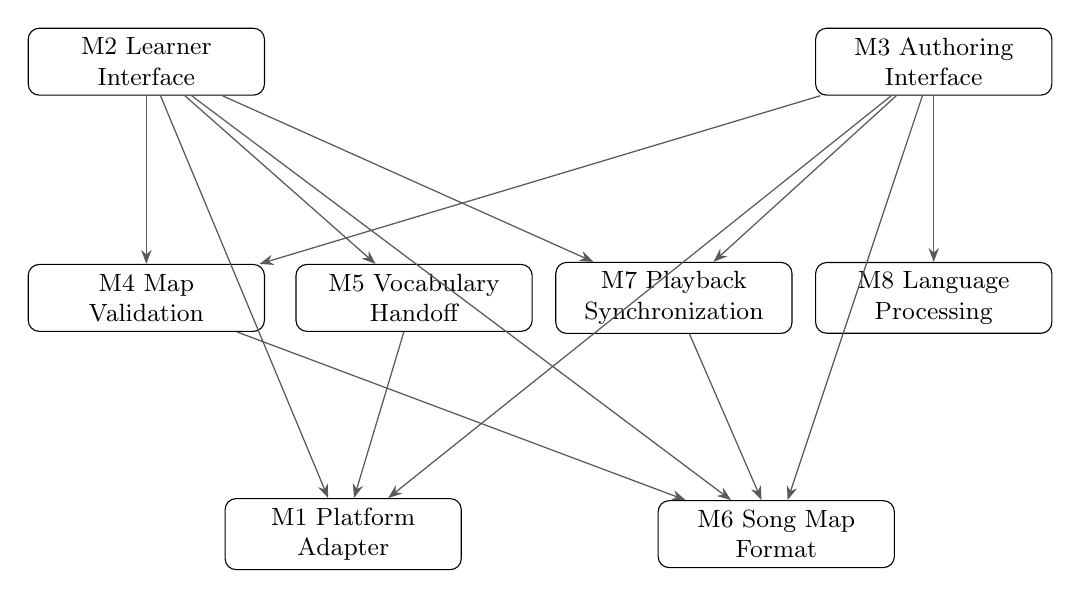
\begin{tikzpicture}[
    >=Stealth,
    box/.style={draw,rounded corners,align=center,minimum width=3cm,
                 minimum height=0.85cm,font=\small},
    edge/.style={->,line width=0.45pt,draw=black!65}
]
\node[box] (learner) at (0,6) {M2 Learner\\Interface};
\node[box] (editor) at (10,6) {M3 Authoring\\Interface};
\node[box] (validator) at (0,3) {M4 Map\\Validation};
\node[box] (handoff) at (3.4,3) {M5 Vocabulary\\Handoff};
\node[box] (sync) at (6.7,3) {M7 Playback\\Synchronization};
\node[box] (language) at (10,3) {M8 Language\\Processing};
\node[box] (platform) at (2.5,0) {M1 Platform\\Adapter};
\node[box] (format) at (8,0) {M6 Song Map\\Format};
\draw[edge] (learner) -- (validator);
\draw[edge] (learner) -- (handoff);
\draw[edge] (learner) -- (sync);
\draw[edge] (learner) -- (platform);
\draw[edge] (learner) -- (format);
\draw[edge] (editor) -- (validator);
\draw[edge] (editor) -- (sync);
\draw[edge] (editor) -- (language);
\draw[edge] (editor) -- (platform);
\draw[edge] (editor) -- (format);
\draw[edge] (validator) -- (format);
\draw[edge] (handoff) -- (platform);
\draw[edge] (sync) -- (format);
\end{tikzpicture}%
}
\caption{Use hierarchy of LingoLyrics modules; arrows point to providers}
\label{FigUH}
\end{figure}

The graph is acyclic. A valid topological layering is
\{\mref{mLearner}, \mref{mEditor}\},
\{\mref{mValidate}, \mref{mAnki}, \mref{mSync}, \mref{mLanguage}\},
and \{\mref{mHH}, \mref{mMap}\}. Lower-level modules do not import
application screens. Dependencies are architectural commitments to be
checked against implementation imports during the Revision~0 review.

%\section*{References}

\section{User Interfaces}

\wss{Design of user interface for software and hardware.  Attach an appendix if
needed. Drawings, Sketches, Figma}

\section{Design of Communication Protocols}

\wss{If there is communication between hardware and software, it may be necessary 
to explain the design of the communication protocol.  This section should be filled 
in with NA if it is not appropriate for a given project.}

\section{Database Design}

\wss{If a database is a significant component of the project, the database
design should be summarized here.  This section should be filled in with NA if
it is not appropriate for a given project.}

\section{Timeline}

\wss{Schedule of tasks and who is responsible}

\wss{You can point to GitHub if this information is included there}

\section{Generative AI Use Disclosure}

\wss{ChatGPT (version 5) was used to brainstorm ideas for the template for this disclose section.}

\subsection{AI Tools Used}

\wss{Give the name of the AI tool(s) used and the version.}

\subsection{How and Where Used}

\wss{Explain what the tool(s) were used for.  Examples include: brainstorming,
explaining a technical concept, reviewing the document, generating or modifying
text, generating or modifying diagrams, identifying errors or omissions or
inconsistencies.}

\wss{For each of the uses, identify which parts of the document were affected.}

\wss{You do not need to report every interaction, but you should disclose the 
uses that materially contributed to your work}

\subsection{Verification of AI-Generated Content}

\wss{\begin{itemize}
    \item Describe how the team checked AI-generated or AI-assisted material
    before including it in the document.
    \item In particular, verify factual claims, technical assertions,
    requirements, calculations, references, and other information for which an
    AI system may produce incorrect or fabricated results.
    \item \textbf{The team is responsible for the accuracy, completeness,
consistency, and appropriateness of the submitted document, regardless of
whether material was generated by a human or an AI system.}
\end{itemize}}

\newpage{}

\bibliographystyle {plainnat}
\bibliography{../../../refs/References}

\end{document}